\section{Design af database} \label{sec:ER}
Det ønskes, at brugerdata er knyttet til den enkelte bruger i databasen. Dette er med henblik på, at app'en ikke skal lagre større mængder data på den mobile enhed samt sikre data i tilfælde af uforudsete hændelser, som eksempelvis tab af mobil enhed. Databasen skal indeholde oplysninger om de enkelte KOL-patienter, herunder resultater opnået ved træning og vennerelation. 

\subsection{ER-diagram}
Modellering af databasen udarbejdes ud fra et ER-diagram. ER-diagrammet relaterer sig til én KOL-patient i databasen. Databasen tager udgangspunkt i entiteter, som sundhedspersonale, KOL-patient, vennerelation, træning og belønninger. ER-diagrammet for databasen fremgår af \autoref{fig:ERdiagram}.

\begin{figure} [H]
\centering
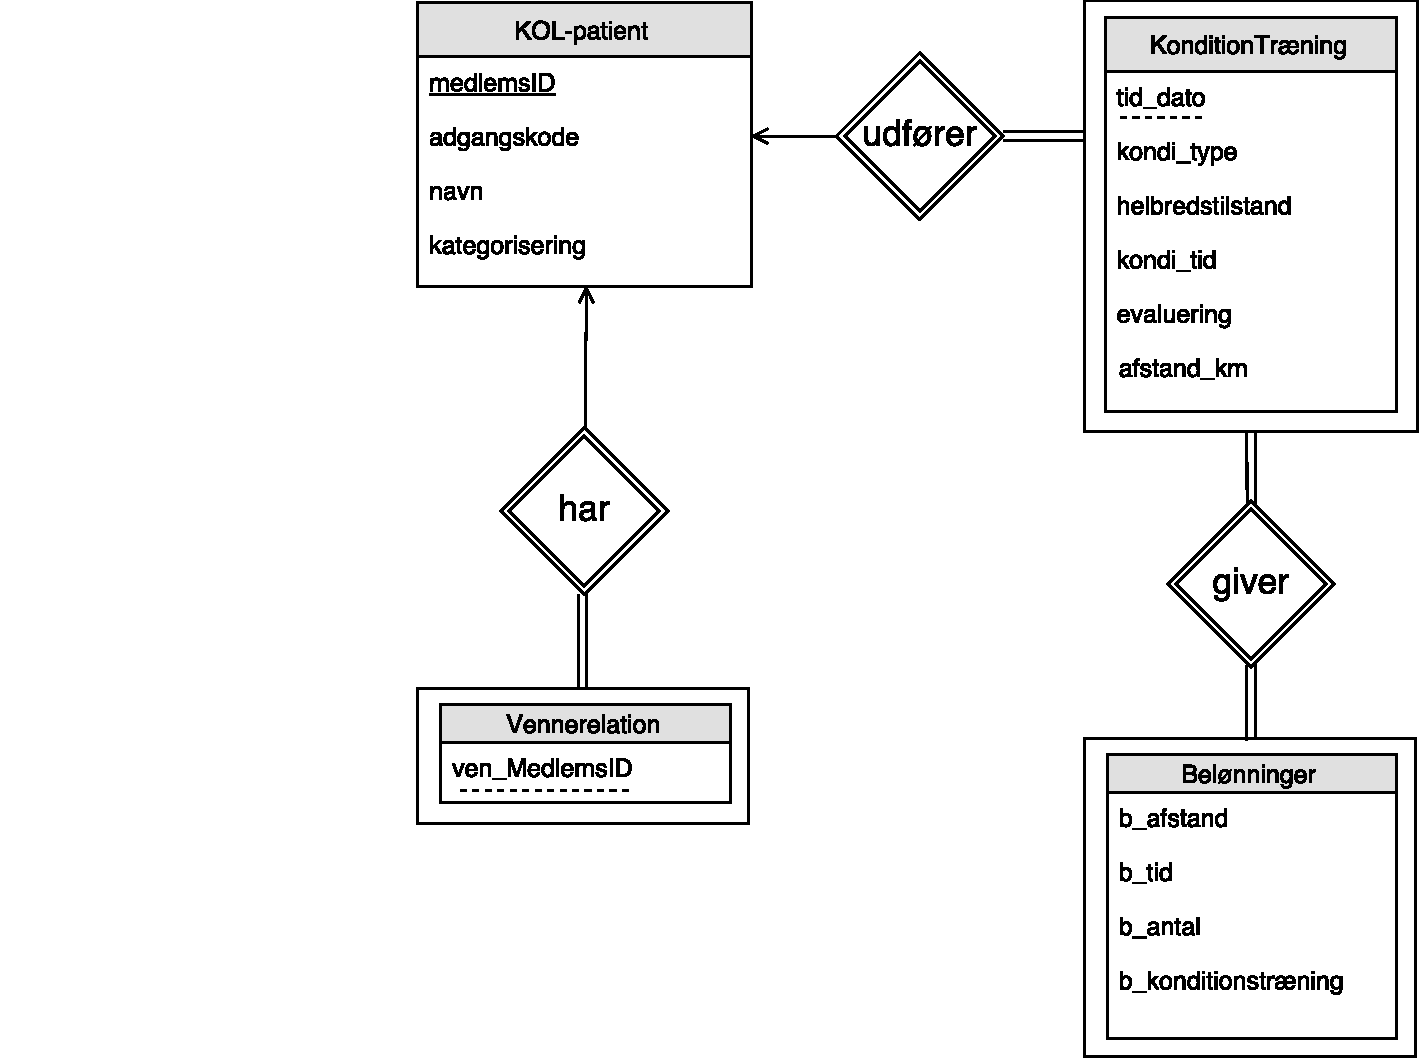
\includegraphics[width=1\textwidth]{figures/Aktivitetsdiagram/ERdiagram}
\caption{ER-diagram for database.}
\label{fig:ERdiagram}
\end{figure} 

\noindent
Af \autoref{fig:ERdiagram} ses ER-diagrammet over databasen, hvori KOL-patienter oprettes og informationer om patienterne samt deres resultater lagres. Sundhedspersonalet fremgår som en stærk entitet, der opretter alle KOL-patienter, hvor én KOL-patient oprettes i databasen én gang. Sundhedspersonalet defineres med et personaleID, afdelingID, personalefornavn og personaleefternavn, hvor \textit{personaleID} er primærnøglen, der kan identificere medarbejderen. Den enkelte KOL-patient er en stærk entitiet, som registreres med primærnøglen, \textit{medlemsID}, samt adgangskode, fornavn, efternavn og kategorisering. Derudover fremgår de svage entiteter, herunder vennerelation, træning og belønninger. Én KOL-patient har mange vennerelationer, som kan identificeres ved KOL-patientens \textit{medlemsID} og \textit{venMedlemsID}. Det samme gør sig gældende for træninger, hvor én KOL-patient kan udføre mange træninger, der identificeres ved  \textit{dato/tid} og \textit{medlemsID}. Ligeledes kan belønninger, som er en mange til mange relation, identificeres ved \textit{data/tid} og \textit{medlemsID}.

\subsection{Schema}
ER-diagrammet omskrives til schema for at kunne normalisere og implementere databasen. Normaliseringen anvendes med henblik på at reducere redundans og inkonsistens. Schema er i anden normalform og fremgår af \autoref{tab:schema}. 

\begin{table} [H]
	\centering
  \begin{tabular}{ | l | p{12cm} |} \hline
     \textbf{Stærke entiteter} & Sundhedspersonale = (\underline{personaleID}, afdelingsID, personaleFornavn, personaleEfternavn)
\newline KOL-patient = (\underline{medlemsID}, adgangskode, fornavn, efternavn, kategorisering) \\ \hline
 	\textbf{Svage entiteter} & Træning = (\underline{medlemsID}, \underline{tid/dato}, træningsform, træningstype, daglig helbredstilstand, tid, afstand, evaluering)
 \newline Vennerelation = (\underline{medlemsID}, \underline{venMedlemsID}, venFornavn, VenEfternavn venBelønninger)
\newline Belønninger = (\underline{medlemsID}, \underline{tid/dato}, afstand, tid, antal, konditionstræning)\\ \hline
    \end{tabular}
    \caption{ER-diagram for databasen omskrevet til schema på anden normalform.}
    \label{tab:schema}
\end{table}


\noindent
Schemaet på anden normalform optimeres til tredje normalform, da det giver bedre muligheder ved implementering af databasen. For at komme på tredje normalform fjernes dimensioner, der ikke har en direkte tilgang til primærnøglen. Tredje normalform ses af \autoref{tab:schema3}.


\begin{table} [H]
	\centering
  \begin{tabular}{ | l | p{12cm} |} \hline
     \textbf{Stærke entiteter} & Sundhedspersonale = (\underline{personaleID}, afdelingsID)
\newline KOL-patient = (\underline{medlemsID}, adgangskode, kategorisering) \\ \hline
 	\textbf{Svage entiteter} & Træning = (\underline{medlemsID}, \underline{tid/dato}, træningsform, træningstype, daglig helbredstilstand, tid, afstand, evaluering)
 \newline Vennerelation = (\underline{medlemsID}, \underline{venMedlemsID},  venBelønninger)
\newline Belønninger = (\underline{medlemsID}, \underline{tid/dato}, afstand, tid, antal, konditionstræning)\\ \hline
    \end{tabular}
    \caption{ER-diagram for databasen omskrevet til schema på tredje normalform.}
    \label{tab:schema3}
\end{table}




